% !TeX encoding = UTF-8
% !TeX root = ../main.tex

%% ------------------------------------------------------------------------
%% Copyright (C) 2021 SJTUG
%% 
%% SJTUBeamer Example Document by SJTUG
%% 
%% SJTUBeamer Example Document is licensed under a
%% Creative Commons Attribution-NonCommercial-ShareAlike 4.0 International License.
%% 
%% You should have received a copy of the license along with this
%% work. If not, see <http://creativecommons.org/licenses/by-nc-sa/4.0/>.
%% -----------------------------------------------------------------------

\section{System architecture}

\subsection{Software application}

\begin{frame}{System architecture}
	\begin{figure}[h]
        \centering
        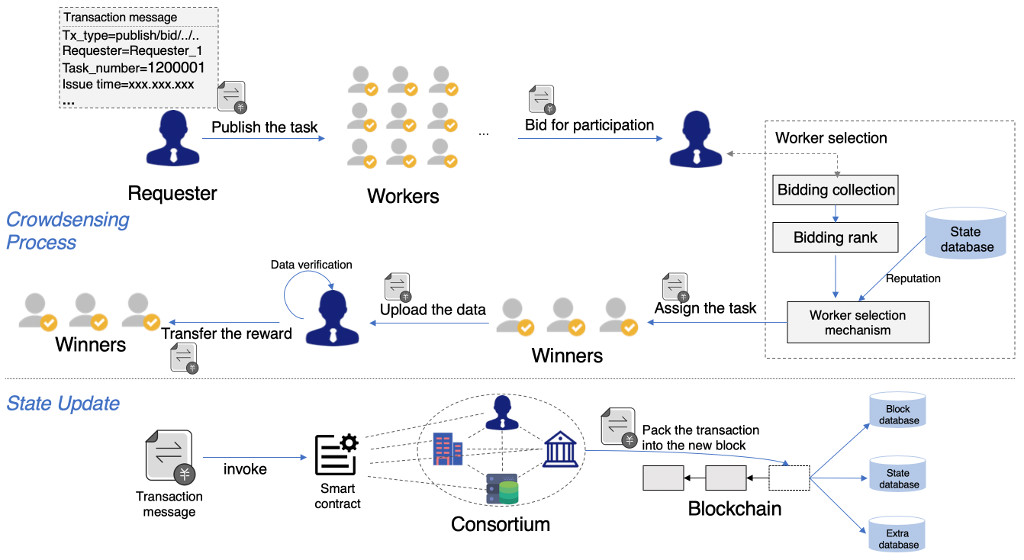
\includegraphics[width=.7\textwidth]{201909-wei-figure2.jpg}
      \end{figure}
\end{frame}

%\begin{frame}{Blockchain application}
%\begin{columns}[T,onlytextwidth]
%    \column{0.7\textwidth}
%	\begin{center}
%		\includegraphics[height=.8\textheight]{eductx.pdf}\hfill
%	\end{center}
%	\column{0.3\textwidth}
%%	\metroset{block=fill}
%      \begin{exampleblock}{Platform}
%        Ethereum
%      \end{exampleblock}
%      \begin{exampleblock}{NF tokens}
%        University credits
%      \end{exampleblock}
%      \begin{exampleblock}{Consensus}
%        Proof-of-stake
%      \end{exampleblock}
%      \begin{exampleblock}{Scope}
%        Public
%      \end{exampleblock}
%      \begin{exampleblock}{Licence}
%        Open source
%      \end{exampleblock}
%\end{columns}
%\end{frame}

%\begin{frame}{Blockchain application}
%  \begin{columns}[c]
%    \begin{column}{.45\textwidth}
%      \begin{itemize}
%        \item Platform
%              \begin{itemize}
%                \item Ethereum
%                \item Hyperledger
%              \end{itemize}
%        \item NF tokens: exchange students
%        \item Consensus: proof-of-stake
%        \item Scope: public
%		\item License: open source
%      \end{itemize}
%    \end{column}
%    \begin{column}{.45\textwidth}
%      \includegraphics[width=\textwidth]{eductx.pdf}
%    \end{column}
%  \end{columns}
%\end{frame}

\begin{frame}{System flow}
  \begin{itemize}
    \item \textbf{System initialization}: configuration and identity authentication mechanisms
    \item \textbf{Task process}: Specific steps of crowdsensing
          \begin{itemize}
            \item Step 1: \alert{Task publishing} (invoking the smart contract to update the task state)
            \item Step 2: \alert{Worker selection} (workers submit the bidding price and workers select appropiate workers)
            \item Step 3: \alert{Data uploading} (selected workers perform the task and upload data)
            \item Step 4: \alert{Reward assignment and data evaluation} (requester distribute rewards and evaluate data quality)
          \end{itemize}
     \item \textbf{System synchronization}: state update about tasks and workers (validating transactions into new blocks)
  \end{itemize}
\end{frame}
